\chapter{Test scenario and evaluation}
\label{chap:testscenarioandevaluation}

In order to evaluate the proposed safety functionality we use the Robostudio version where we already integrated LTLCreator in. This visual programming environment allows the specification of state machine based programs whose behaviour can then be examined by visual constraints.
As a test scenario we consider the simplified medication reminder application whose underlying screen-flow is explained in figure~\ref{fig:medicationreminder}. Starting from ``Menu'' the user can choose from several services such as blood pressure measurement or entertainment. In the given example these services are simplified to just one state ``additional services'' since we want to focus only on the medication reminder part. In ``Polling'' the database is checked for a pending reminder, and if there is one the medication intake guidance is triggered. The patient can state if he or she has already taken the medication, or decide whether to take it or not. In the latter he or she may give a reason for it and a caregiver is notified about this incident. Otherwise it will result in ``Well done!'' after completing intake.

\begin{figure}[htbp]
  \centering
  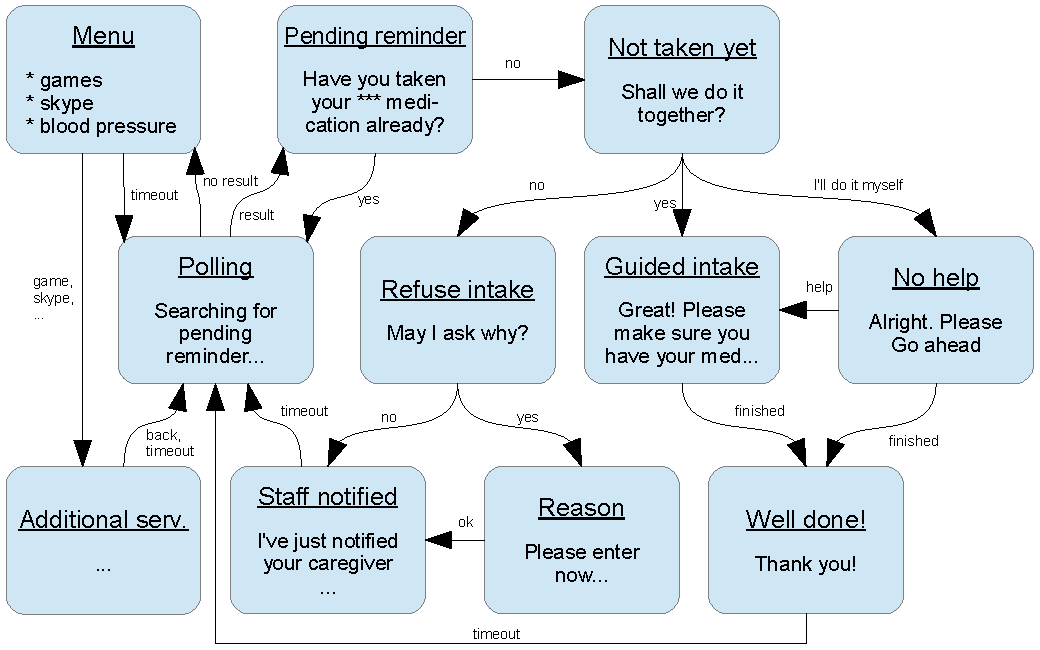
\includegraphics[width=\linewidth]{stm.pdf}
  \caption{Simplified screen-flow of the medication reminder application.}
  \label{fig:medicationreminder}
\end{figure}

This state machine with all its states, transitions and screen dialogs has been implemented in Robostudio and in the following sections we will evaluate the visual language as well as the capability of constraint generation. In section~\ref{sec:practicalexperiences} it is described how a non-expert deals with the visual language and what the final judgement is.



\section{Operator constraints}

Before we can start creating constraints it might be useful to think about a reasonable term we want to express. Let's take the example ``Whenever there is a pending reminder, medication will be finally taken or caregivers will get notified in case of the patient refusing medication intake.'' given as a requirement in chapter~\ref{chap:goals}.

In order to find a corresponding graphical constraint the sentence has to be analyzed just as you read it. Since ``whenever'' is a semantic equivalent to ``always if'' first of all a \emph{ALWAYS} operator gets dragged to the dashboard directly followed by an \emph{IF} as shown in figure~\ref{fig:sampleconstraint}. The condition for this \emph{IF} is that there is a pending reminder, so a state ``Not taken yet'' has to be added to the upper bucket of the \emph{IF} operator.
Whenever the just mentioned condition becomes true, there also has to be true in future: Medication is taken properly or caregivers get notified about refuse. Accordingly a \emph{FUTURE} operator containing an \emph{OR} forms the second part of the \emph{IF} operator. Finally two states 'Well done!' and 'Staff notified' get added to the disjunction. The resulting visual constraint can now automatically be translated to the corresponding LTL formula by the editor:

\begin{equation} \label{eq:sampleconstraint}
  \models \Box (\textnormal{'Not taken yet'} \Rightarrow \Diamond (\textnormal{'Well done!'} \vee \textnormal{'Staff notified'}))
\end{equation}

\begin{figure}[htbp]
  \centering
  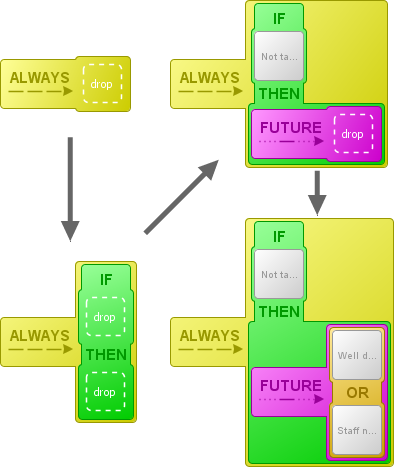
\includegraphics[scale=0.65]{sampleconstraint}
  \caption{Visual constraint creation for LTL formula ~\ref{eq:sampleconstraint}.}
  \label{fig:sampleconstraint}
\end{figure}

After each change in the dashboard, the constraint is automatically recompiled and revalidated by using the underlying model checker. For syntactically invalid constraints, an ``incomplete'' sign is displayed in the respective tab. Otherwise, an animated ring indicates that validation is in pro\-gress and will finally result in either a ``valid'' or ``invalid'' sign.

Due to the optimized performance of NuSMV, even the validation of constraints on huge and complex programs is fast and allows rapid feedback. In addition, the validation itself runs in the background without locking the dashboard. Therefore we avoid waiting times and disruptions during constraint development, which would be likely with conventional model checking where constraint development and constraint validation are alternating processes. Thus we consider our tool an improvement for the user experience.

We observed the different color flavours of the visual operators to be a good support for fast reading and understanding of constraints. Also the two dimensional composition and the round shapes of the operators turned out to 
give the language a schematic but not too rectangular look. Besides it is considered eye-candy what is the best motivation for using this visual language.





\subsection{Expressiveness}

Due to its basing on LTL, the visual language's expressivenes is equivalent to LTL's one of course. More precisely this means any logic formula can be expresssed except potentiality.
Furthermore there is one more limitation in the current visual language with the variety of available proposition operators. The visual language was originally designed for validating healthcare applications where just one kind of proposition is needed: ``currently state x is active''. Thus other propositions such as equations, greater than etc. are not implemented yet, but can be easily extended.
Figure~\ref{fig:example_propositions} depicts how an extention of \emph{LTLCreator} with additional proposition operators could be realised.

\begin{figure}[htbp]
  \centering
  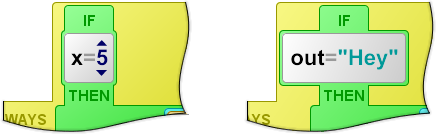
\includegraphics[scale=0.65]{example_propositions}
  \caption{Possible proposition extensions: numeric and string equations.}
  \label{fig:example_propositions}
\end{figure}



\section{Automated constraint generation}

The automated constraint generation can be triggered by a click on the magic wand button in the tab area. After activation a dashboard is opened in a new tab for each found constraint, and validation is initiated immediately. For the medication reminder application six constraints are found, including \emph{a)} and \emph{b)} shown in figure~\ref{fig:generatedconstraints} which match the postulations in the requirements in chapter~\ref{chap:goals}.
The constraint used for demonstration in the previous section is also generated, however \emph{b)} forms an intensified restriction of it. 
Constraint \emph{a)} ensures the ``Polling'' state is always eventually visited again. If a pending medication is not already taken, constraint \emph{b)} guarantees intake or staff notification before the next reminders can be read from the database.

The search and generation process finishes within less than a second and thus doesn't make the developer wait for a long time.

We showed that the subgraph approach is working for the medication reminder application, and there was even one more reasonable constraint found by the heuristic: Constraint \emph{c)} ensures that during the medication intake process the program can not switch back to the menu or other services such as entertainment or blood pressure measurement.



\begin{figure}[htbp]
  \centering
  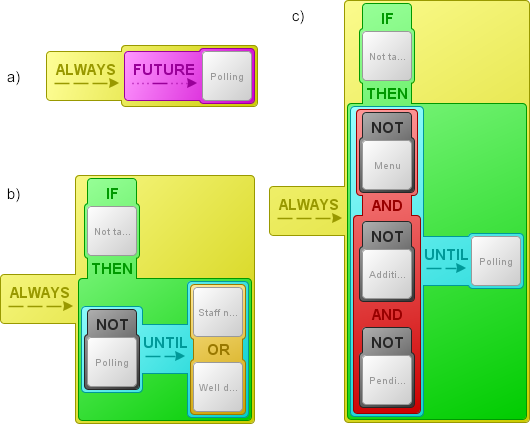
\includegraphics[scale=0.65]{generatedconstraints}
  \caption{Automatically generated constraints which match the required postulations.}
  \label{fig:generatedconstraints}
\end{figure}






\subsection{Performance}

In order to examine the performance of subgraph finding and constraint generation, we need to have a second look at the implementation details again. The subgraph finding algorithm is realized as a depth-first search. Indeed all healthcare programs are infinite and contain cycles and a depth-first walk-through would never end, but the algorithm doesn't go deeper at already visited states.

The performance of this algorithm is of course highly dependend on the grade of branching. Nevertheless, such a depth-first search has an estimated wost case execution time of $O(|V|+|E|)$ in which $|V|$ is the number of states and $|E|$ number of edges respective transitions in our case.
Since we cope with state machines and thus have directed edges rather than undirected ones, each state can have $|V|$ transitions; $|V-1|$ to other ones and one to itself. For the contained tree without cycles for depth-first search we retreive $|E|=|V|$ edges.
As worst case ececution time for the depth-first search we obtain the following result:

\begin{equation}
O(\textnormal{``depth-first search''})=O(|V|)+O(|V|-1)=O(|V|)
\end{equation}

In order to find a subgraph with our presented algorithm the depth-first search has to be startet on a start state of a subgraph. Since we don't know in beforehand which states might be possible candidates for such start states, the algorithm has to be applied on every single state of the program which has two ore more outgoing transitions. In the worst case all $|V|$ states match this condition, so the depth-first search has to be executed $|V|$ times. This implies for our estimated worst case execution time:

\begin{equation}
O(\textnormal{``subgraph finding''})=O(|V|)*O(|V|)=O(|V|^2)
\end{equation}



\subsection{Scalability}

For all the healthcare applications the presented algorithm works efficient and fast. But their program sizes are still quite manageable. Our test program has eleven states, an average branch grade and a constraint finding execution time of a split second on a standard pc.
Of course an exponential execution time is bad if the number of states arises. A clear slowdown can be felt when the algorithm runs on larger state machines with plenty of states and high grade of branching. A test on a state machine with over two hundred and fifty states and partially high branch grade resulted in approximately five minutes execution time.

However, sholud this algorithm regardless its tailoring to the healthcare domain be used for other huge programs, it keeps a lot of potential to be improved in efficiency. With a sophisticated approach it might be enough to execute just one depth-first search for finding all subgraphs at once what would lead to a linear execution time.
% wenn noch schreiben will, dann: linear ist cool, weil das tool eh die gefundenen constraints gleich anzeigt und nicht erst am ende alles geballt bringt.


\subsection{Reasonability of generated constraints}

The constraint generator algorithm found six constraints for the medication reminder application. Two of them were actually the ones we proposed in the requirements. Three of them are either intensified versions of the previous ones or just describe the behaviour of the program and thus make sense, but in matters of safety they aren't fundamental relevant.
Nevertheless the generator tool actually helped us in finding a new important constraint we didn't think about before.

To put it in a nutshell, all automatically generated constraints are practical, and approximately half of them are significant. We showed that the constraint generator concept works well for the healthcare application and can be a very helpful feature.




\section{Practical experiences}
\label{sec:practicalexperiences}

eher schreiben: wurde einigen Leuten vorgestellt. Generell blabla... Darunter auch alina kracker...

Alina Kracker, 21 Jahre alt aus Friedberg und Studentin der Erziehungswissenschaften, arbeitet neben dem Studium als Pflegehilfskraft in einer Kurzzteitplfege. Dort betreut sie �ltere Damen und Herren, die dort kurz- bis mittelfristig untergebracht sind. In dieser Einrichtung wohnen Personen mit unterschiedlichsten Krankheiten und Bed�rfnissen, von zu beobachtenden aber gesunden Menschen bis hin zu Alzeimerpatienten.

Es wurde getestet, ob Kracker ohne entsprechende Ausbildung Constraints zu dem Beispiel des medication reminder formulieren kann.
Zum einen m�chte die Universit�t of Auckland die Programmierung solcher Anwendungen auch nicht-professionellen erm�glichen, und da w�re die Erfahrung einer echten Pflegekraft mit dieser Aufgabe wohl sehr interessant. Zum anderen kann so aber auch festgestellt werden, wie nicht-Softwareentwickler mit der visuellen Sprache und dem Konzept zur Constrainterstellung zurechtkommen.

Kracker wurde in das Beispiel der medication reminder applikation eingef�hrt und das Programmverhalten anhand der Zustandsmaschine aus figure 123 erkl�rt. Anschlie�end wurde sie mit der Oberfl�che und Funktionsweise des LTLCreator tools vertraut gemacht.

Ihr wurde nun die Aufgabe gegeben, mit den im Editor zur Verf�gung stehenden Mitteln die zwei Bedingungen zu formulieren, die uns in diesem Kapitel bereits begleitet haben. Zum einen sollen Medikamenterinnerungen nie vergessen werden, also Zustand ``Polling'' muss regelm��ig besucht werden. Zum anderen muss sichergestellt sein, dass bei noch nicht vorgenommener Medikamenteinnahme das Medikament letztendlich eingenommen wird oder das Personal benachrichtigt wird. Also bei Besuch von ``Not taken yet'' muss entweder ``Well done!'' oder ``Staff notified'' besucht werden.

Da Kracker mit Zustandsmaschinendarstellungen nicht vertraut ist, wurden ihr die Constraintbedeutungen wie eben beschrieben anhand der Zustandsnamen erl�utert. Bei der Erstellung der Constraints war sie allerdings anf�nglich auf sich alleine gestellt. Die erste Bedingung erstellte sie z�gig und richtig, und es schien auch keine besondere Herausforderung gewesen zu sein. 
Auch der zweite Constraint wurde
Bei der Frage nach der Anwendung von FUTURE hakte es dann allerdings etwas, was auf die zeitlichen (...) zur�ckzuf�hren war. Die Aufforderung, die Bedingung als deutschen Satz zu formulieren, half ihr wieder auf die Spr�nge.

F�r eine Person, die von modelchecking oder LTL noch nie etwas geh�rt hat, kam sie mit kleinen Hilfen gut mit der visuellen Sprache zurecht und k�nnte sie so mit etwas �bung auch verwenden.

Die N�he zwischen LTL und deutschem Satz ist gut, und dadurch kann man schnell konstraints zusammen klicken (besser als mit fremden mathematischen symbolen).


Auf die Frage, ob sie solche Roboteranwendungen wie der Medicationreminder in der Kurzzeitpflege f�r sinnvoll erachten w�rde, antwortet Kracker: ``F�r geistig fitte aber dennoch vergessliche und t�telige Leute kann ich mir diese Roboterapplikation super vorstellen. Ein Gro�teil unserer Patienten ist jedoch nicht in der Lage Entscheidungen, die der Roboter abfr�gt, wahrheitsgem�� zu treffen. Aufgrund der regelm��ig wechselnden Patientenbelegung in der Kurzzeitpflege ist es vielmehr f�r das Betreuungspersonal eine gro�e Herausforderung, die uhrzeitgebundenen Medikamenteinnahmen der Patienten nicht zu vergessen. Daher w�re eine solche Erinnerungsfunktion f�r das Personal eine gro�e Hilfe.''.